\section{Platinum---Berry curvature-like term and spin Hall conductivity}
\label{sec29:PtSHC}

\begin{itemize}
	\item Outline: {\it Calculate the Berry curvature-like term and spin Hall conductivity
	of fcc Pt with spin-orbit coupling. In preparation for this example it may be useful to read Ref.~\onlinecite{qiao-prb2018} and Ch. 12 of the User Guide.}
\end{itemize}

\begin{itemize}
	\item[1-6] {\it Compute the MLWFs and compute the {\tt kpath}, {\tt kslice} and spin Hall conductivity.} 
\end{itemize}

\subsection*{Berry curvature-like term plots}
\begin{itemize}
	\item {\it The band-projected Berry curvature-like term $\Omega_{n,\alpha\beta}^{\text{spin} \gamma}({\bm k})$ 
		is defined as Eq.~(12.22) of the User Guide.}
	{\it Plot the band structure of Pt and color it 
		by the magnitude of its band-projected Berry curvature-like term $\Omega_{n,xy}^{\text{spin}z}(\bf k)$, 
		and plot the k-resolved Berry curvature-like term $\Omega_{xy}^{\text{spin}z}(\bf k)$ along the 
		same path in the BZ. }

	The calculated Fermi energy is $17.9919$ eV. It may vary among different calculations due to the difference between versions of {\tt Quantum ESPRESSO} or compilers, and these may lead to deviations from the following results. However, the difference should be small and the calculated SHC should be essentially the same. With this value we obtain the energy bands colored by the 
	$\Omega_{n,\alpha\beta}^{\text{spin} \gamma}({\bm k})$ and the k-resolved Berry curvature-like term $\Omega_{xy}^{\text{spin}z}(\bf k)$ along high-symmetry points shown in \Fig{fig29.1}. 
	In the following two plots with different fixed smearing width are shown.
\end{itemize}

\begin{figure}[htb!]
\centering
\subfloat[With fixed smearing of 1 eV]{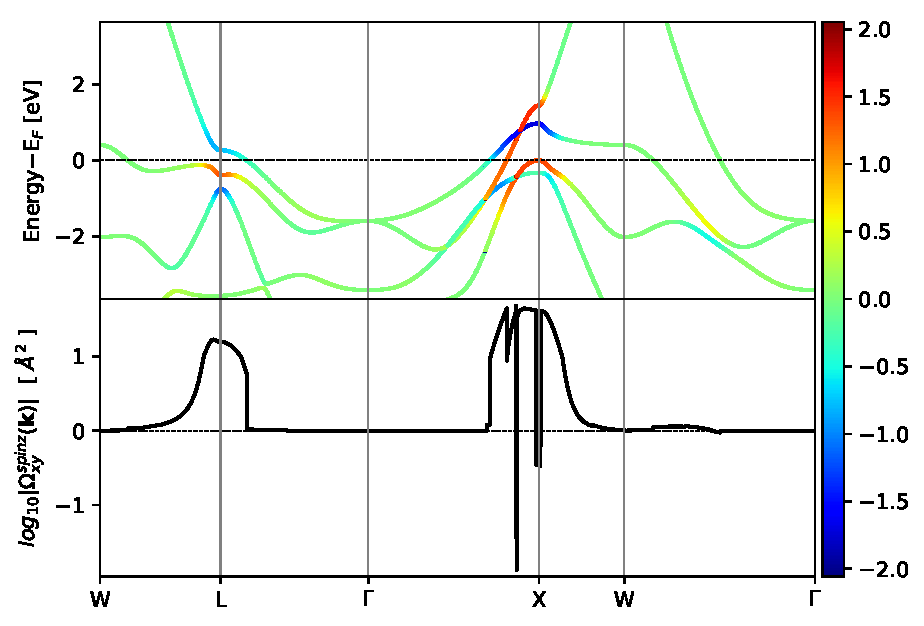
\includegraphics[width=0.45\columnwidth]{figure/example29/Pt-bands+shc_1.pdf}}\qquad
\subfloat[With fixed smearing of 0.05 eV]{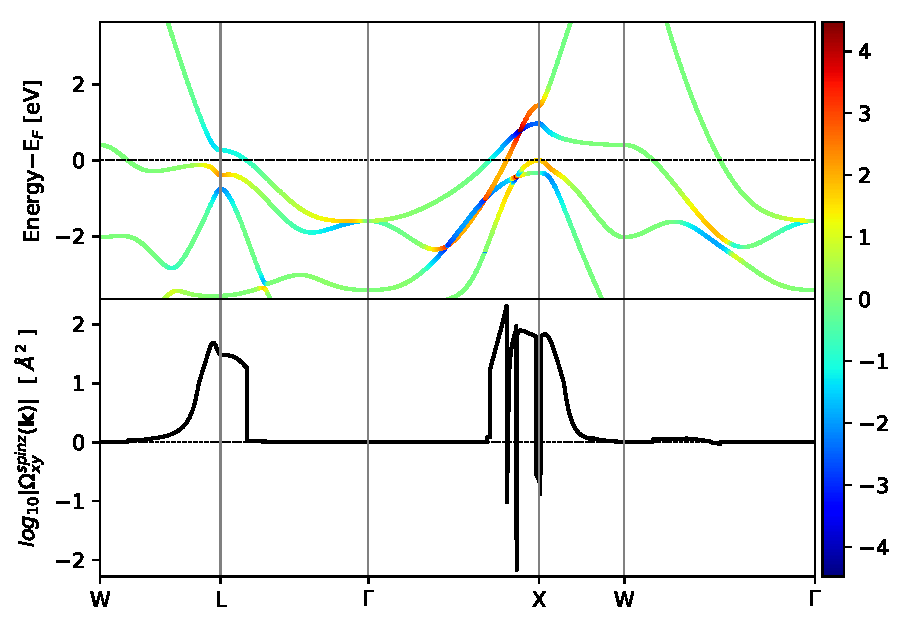
\includegraphics[width=0.45\columnwidth]{figure/example29/Pt-bands+shc_0_05.pdf}}
\caption{Top panel: Band structure of Pt along symmetry lines W-L-$\Gamma$-X-W-$\Gamma$, colored by
the $\Omega_{n,xy}^{\text{spin}z}({\bm k})$. 
Bottom panel: k-resolved Berry curvature-like term $\Omega_{xy}^{\text{spin}z}(\bf k)$ along the symmetry lines.}
\label{fig29.1}
\end{figure}
\clearpage

\begin{itemize}
	\item {\it Combine the plot of the Fermi lines on the $k_y$ plane with a heatmap plot of the Berry curvature-like term of SHC.}

	The plots of the Fermi lines with a colormap of $\Omega_{xy}^{\text{spin}z}(k_x,0,k_z)$ are shown in \Fig{fig29.2}.
\end{itemize}

\begin{figure}[htb!]
	\centering
	\subfloat[With fixed smearing of 1 eV]{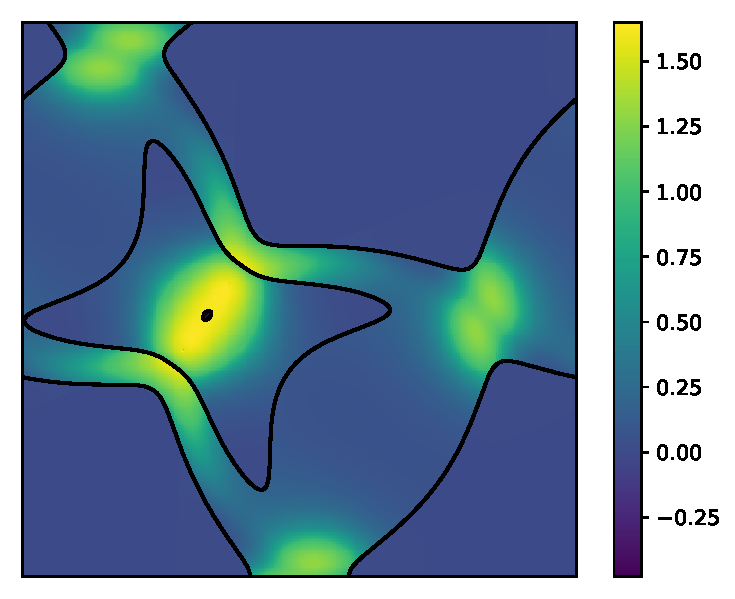
\includegraphics[width=0.45\columnwidth]{figure/example29/Pt-kslice-shc_1.pdf}}\qquad
	\subfloat[With fixed smearing of 0.05 eV]{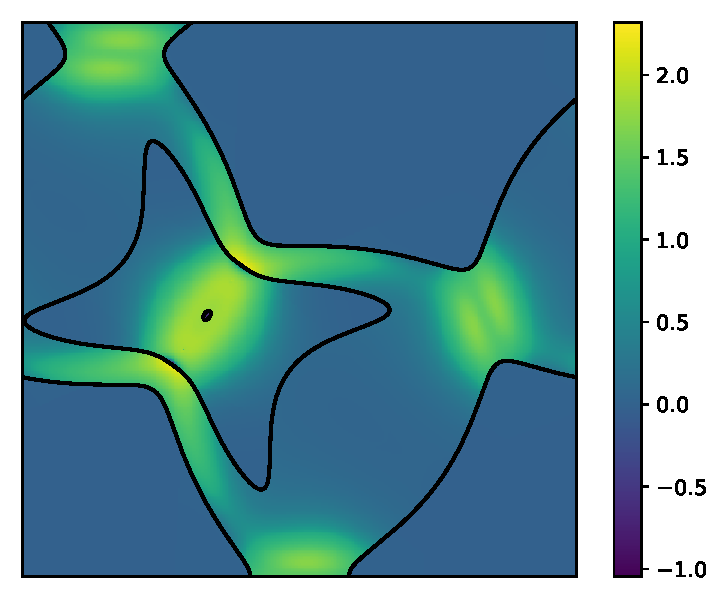
\includegraphics[width=0.45\columnwidth]{figure/example29/Pt-kslice-shc_0_05.pdf}}
	\caption{Calculated k-resolved Berry curvature-like term $\Omega_{xy}^{\text{spin}z}(\bfk)$ in the plane $k_y=0$ (note log scale). Intersections of the Fermi surface
		with this plane are shown.}
	\label{fig29.2}
\end{figure}

\clearpage
\subsection*{Spin Hall conductivity}

\begin{itemize}
	\item {\it SHC converges rather slowly with k-point sampling, and a $25 \times 25 \times 25$ does not yield a well-converged value.
	Compare the converged SHC value with those obtained in Refs.~\onlinecite{qiao-prb2018} and \onlinecite{guo-prl2008}.}

	The file {\tt Pt-shc-fermiscan.dat} contains the calculated SHC. The SHC for a $25\times25\times25$ BZ mesh are shown in the snippet below. The SHC 
	at the Fermi energy (17.9919 eV) is 1705 $\frac{\hbar}{e}\mathrm{S/cm}$. 
	The converged result reported in Refs.~\onlinecite{qiao-prb2018} and \onlinecite{guo-prl2008} is around 2200 $\frac{\hbar}{e}\mathrm{S/cm}$. Hence, a $25\times25\times25$ BZ mesh clearly gives a very inaccurate value ($\sim 22.5\%$ error).   

\begin{tcolorbox}[title=$25\times25\times25$ kmesh,sharp corners,boxrule=0.5pt]
{\small
\begin{verbatim}
#No.   Fermi energy(eV)   SHC((hbar/e)*S/cm)
   1     6.000000    0.00000000E+00
...
 120    17.900000    0.17230482E+04
 121    18.000000    0.17054542E+04
...
 201    26.000000    0.22665760E+03
\end{verbatim}
}
\end{tcolorbox}

Since these are quite demanding calculations, we only report the value of the SHC for a $100\times100\times100$ BZ mesh (see snippet below). The value for the SHC is 2207 $\frac{\hbar}{e}\mathrm{S/cm}$, which is in much closer agreement with the converged result from Refs.~\onlinecite{qiao-prb2018} and \onlinecite{guo-prl2008}.

\begin{tcolorbox}[title=$100\times100\times100$ kmesh,sharp corners,boxrule=0.5pt]
{\small
\begin{verbatim}
#No.   Fermi energy(eV)   SHC((hbar/e)*S/cm)
   1     6.000000    0.00000000E+00
...
 120    17.900000    0.21899191E+04
 121    18.000000    0.22066678E+04
...
 201    26.000000    0.24919920E+03
\end{verbatim}
}
\end{tcolorbox}

\item To complete the previous discussion, we also 
compare the Fermi energy scan plots of the two calculations in the \Fig{fig29.3}. 
\begin{figure}[htb!]
\centering
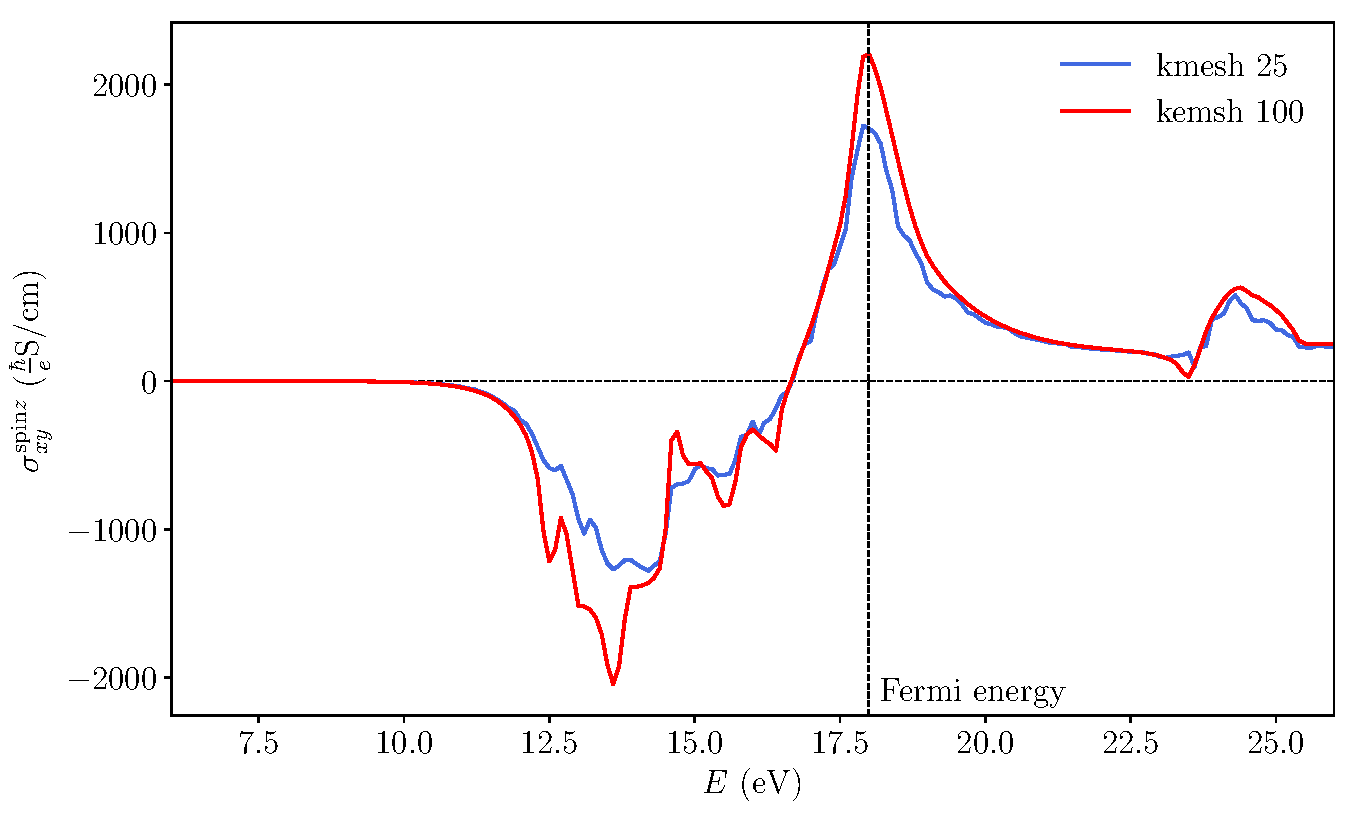
\includegraphics[width=.8\columnwidth]{figure/example29/pt_shc_kmesh.pdf}
\caption{Fermi energy scan plots for calculations 
	with $25\times25\times25$ and $100\times100\times100$ kmeshes.}
\label{fig29.3}
\end{figure}

\item The {\tt seedname.wpout} will print the percentage of k-points which 
have been calculated at the moment, as well as the corresponding calculation time, as 
shown in the following snippet. 
This might be helpful as you can roughly 
estimate the total computational time 
of your calculation, or it might give credence to the code that it is actually functioning :). 
Note this report is merely based on the ``root'' computation node. It is accurate if the {\tt postw90} is run in serial, or the load on each node is balanced if running in parallel. However, the estimation is rough if loads are not balanced among nodes. This may happen if the performance of nodes in your cluster are not identical, or adaptive k-mesh refinements are triggered so some nodes may compute much more k-points than others. 
Besides, if you are careful enough, you may find the diff time of 10\% is much larger than later ones. This 
is caused by some done-once-and-for-all computations carried out at the beginning, thus 
later computations are much faster. 
\begin{tcolorbox}[title=Pt.wpout,sharp corners,boxrule=0.5pt]
{\small
\begin{verbatim}
 Properties calculated in module  b e r r y
 ------------------------------------------

   * Spin Hall Conductivity

     Fermi energy scan
 
 Calculation started
 -------------------------------
   k-points       wall      diff
  calculated      time      time
  ----------      ----      ----
       0%          0.0       0.0
      10%         22.7      22.7
      20%         36.5      13.8
      30%         50.4      14.0
      40%         64.4      14.0
      50%         78.4      14.0
      60%         92.5      14.1
      70%        106.5      14.0
      80%        120.4      13.9
      90%        134.2      13.8
     100%        147.9      13.7


 Interpolation grid: 25 25 25

 Using adaptive smearing
       adptive smearing prefactor    1.414
       adptive smearing max width    1.000 eV
       
\end{verbatim}
}
\end{tcolorbox}

\end{itemize}

